\documentclass[table,svgnames]{beamer}
\usepackage{mathabx}
\usepackage{mathrsfs}
%\usepackage{eulervm}
\usepackage{units}
\usepackage{calc}
\usepackage{tikz}
\usepackage[alpine]{ifsym}
\usepackage{marvosym}
\usepackage[normalem]{ulem}
\usetikzlibrary{arrows,automata,mindmap,patterns,shapes,snakes,trees}

\hypersetup{
	pdfkeywords={Trusted Platform Module, Software-Based Emulator, TPM,
		Trusted Computing},
	pdfpagemode={FullScreen}
}

\newtheorem*{proposition}{Proposition}

\mode<presentation>
{
	\usetheme{default}
	\usefonttheme[onlylarge]{structurebold}
	\usefonttheme[onlymath]{serif} % for Euler font
	
	%\setbeamertemplate{blocks}[rounded]
	\setbeamertemplate{navigation symbols}{}
	\setbeamertemplate{itemize items}{\textcolor{structure}{
		$\sqbullet$}}
	\setbeamertemplate{enumerate items}[square]
	%\setbeamertemplate{theorems}[numbered]
	\setbeamercolor{block title}{fg=structure,bg=gray!25}%
	\setbeamercolor{block body}{parent=normal text,bg=gray!10}%
	\setbeamercolor{block title example}{bg=gray!30!green!30}%
	\setbeamercolor{block body example}{parent=normal text,bg=gray!15!green!15}%
  
  \setbeamercovered{transparent}
}

\title[TPM Emulator]{A Software-Based\\
	Trusted Platform Module Emulator}

\author[M. Strasser, H. Stamer]{
	\textbf{Mario Strasser}\inst{1}
	\and
	\underbar{\textbf{Heiko Stamer}}\inst{2}}

\institute[ETH Zurich, Uni Kassel]{
	\inst{1}
		ETH Z{\"u}rich, Switzerland\\
		\texttt{strasser@tik.ee.ethz.ch}
	\and
	\inst{2}
		Universit{\"a}t Kassel, Germany\\
		\texttt{stamer@theory.informatik.uni-kassel.de}\\
		{\tiny\texttt{76F7 3011 329D 27DB 8D7C\quad  3F97 4F58 4EB8 FB2B E14F}}}

\date[TRUST 2008 (Villach)]{TRUST 2008, Scientific Conference on
	Trusted Computing\\
	Villach, Austria, March 11--12, 2008}

\subject{Trusted Computing}

% Falls eine Logodatei namens "university-logo-filename.xxx" vorhanden
% ist, wobei xxx ein von latex bzw. pdflatex lesbares Graphikformat
% ist, so kann man wie folgt ein Logo einf�gen:

\pgfdeclareimage[height=0.5cm]{unik-logo}{uniklogo}
\pgfdeclareimage[height=1cm]{ethz-logo}{ethlogo_black}
\logo{\raisebox{-2mm}{\pgfuseimage{ethz-logo}}\hspace{6.5cm}\pgfuseimage{unik-logo}}

% Falls Aufz�hlungen immer schrittweise gezeigt werden sollen, kann
% folgendes Kommando benutzt werden:

%\beamerdefaultoverlayspecification{<+->}

\begin{document}

\begin{frame}
	\titlepage
\end{frame}

\logo{}

\begin{frame}
	\frametitle{Outline}
	\tableofcontents
\end{frame}

%\renewcommand{\pause}{}

\section{Motivation}

\begin{frame}
	\frametitle{Why emulating a TPM in software?}
	TPM emulator has been proved to be useful in various ways, e.g.,
	\begin{itemize}
		\item to run more than one TPM instance per platform\\
			(\alert{\emph{virtualisation}}),
			\begin{itemize}
				\item Hewlett-Packard: Trustworthy Virtualisation Environment
				\item VMKnoppix (Xen Hypervisor), patch for \textsc{QEMU}, \ldots
			\end{itemize}\pause
		\item to restore previously stored or artificially created states\\
			(\alert{\emph{testing}}, \alert{\emph{debugging}}, and 
			\alert{\emph{educational purposes}}),
			\begin{itemize}
				\item TU Graz: class ``AK IT-Sicherheit 1 / Trusted Computing''
			\end{itemize}\pause
		\item to simulate new TPM commands and vendor extensions\\
			(\alert{\emph{research}} and \alert{\emph{development}})
			\begin{itemize}
				\item Princeton University, NEC, Texas Instruments: energy and
					execution time analysis of ECC algorithms (DATE 2007)
				\item Nokia: Validation of MTM specification (MTM Emulator)
			\end{itemize}\pause
	\end{itemize}
	Of course, a software-based TPM cannot provide the same security
	guarantees (tamper-resistance, trust anchor) like a hardware chip.
\end{frame}

\begin{frame}
	\frametitle{Basic Facts}
	\begin{description}[]
		\item[Project Goal:] Create a working software-based TPM emulator
			that is compliant with TCG TPM specification version 1.2
		\item[Supported Operating Systems:] GNU/Linux, Open/FreeBSD, \ldots
			(ebuild script for Gentoo Linux available)
		\item[Last Stable Version:] 0.5.1 (2008-02-12), GPL v2,
			${}\approx 25$k LOC
		\item[Development Site:] \url{https://tpm-emulator.berlios.de/}
    \item[Prerequisites:] \texttt{/dev/urandom} or similar, Unix domain sockets
		\item[Third-Party Libraries:] GNU Multiple Precision Arithmetic Library
			(bignum support for RSA and DAA)
		\item[History and Milestones:]\hfill\\
			\begin{itemize}
				\item 2004: Started by Mario Strasser as semester thesis
				\item 2005, Apr.: Session management and RC4 encryption added
				\item 2005, Dec.: Identity functions and DAA support added
				\item 2006, Dec.: Milestone version 0.5 released
			\end{itemize}
	\end{description}
\end{frame}

\section{Design and Implementation}

\begin{frame}
	\frametitle{Design and Implementation}
	\begin{description}[]
		\item[New Design:] User-space daemon \texttt{tpmd}
			(since version 0.5)\\
			\begin{center}
				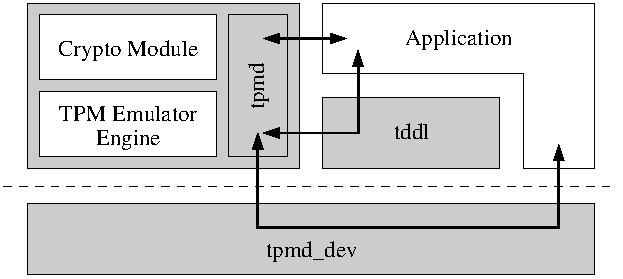
\includegraphics[width=.95\textwidth]{figures/system_overview}
			\end{center}\pause
		\item[Accessing the Emulator:]\hfill\\
			{\small\begin{enumerate}
				\item Direct (Unix domain socket \texttt{/var/run/tpm/tpmd\_socket:0})
				\item Recommended (TDDL interface according to TSS spec.)
				\item Legacy (Linux/BSD kernel module \texttt{tmpd\_dev} provides
					\texttt{/dev/tpm})
			\end{enumerate}}
	\end{description}
\end{frame}

\begin{frame}[fragile]
	\frametitle{Design and Implementation}
	\begin{description}[]
		\item[Implementation Issues:]\hfill\\
			{\small\begin{itemize}
				\item Up to version 0.4.1 the TPM emulator was a Linux kernel module:
				\begin{itemize}
					\item Kernel stack size is very limited (4 KB resp. 8 KB on x86)
					\item Debugging was very difficult (call paths with stack overflows)
					\item Persistent storage needed for executing \textsf{TPM\_SaveState}
					\item Command serialization and synchronization by semaphores
				\end{itemize}
				\item Alignment of structures and bignums in combination with hashing
				\item Typographical errors and ambiguities in the TPM specification:
				\begin{itemize}
					\item
{\tiny ``\verb|TPM computes a TPM-specific secret f0 (104-bit) = f mod 2104|''
(Part 1, rev 94)}
				\item
{\tiny ``\verb|#define DAA_SIZE_r3 158|'' (Part 2, rev 62) \hspace{3mm}
``\verb|#define DAA_SIZE_r3 168|'' (Part 2, rev 85)}
				\item
{\tiny ``\verb|obtain DAA_SIZE_NT bits from RNG|'' (20 bits vs. 20 bytes)
(Part 3, rev 94)}
			\end{itemize}
			\end{itemize}}\pause
		\item[Tools and Helpers:]\hfill\\
			{\small\begin{itemize}
				\item Automatically generated (un)marshalling code (Perl, awk, sed)
				\item Testing TPM command request structures by using IBM's
					\texttt{buildbuff}-function from \texttt{tpm-3.2.0/libtpm/tpmutil.c}
			\end{itemize}}
	\end{description}
\end{frame}

\section{Performance Evaluation}

\begin{frame}
	\frametitle{Performance Evaluation (1)}
	\begin{description}[]
		\item[Evaluation Environment:] IBM ThinkPad T43p (Intel Pentium M 2\,GHz,
			1 GB RAM), Linux 2.6.23, NSC TPM v1.1b
			\begin{center}
				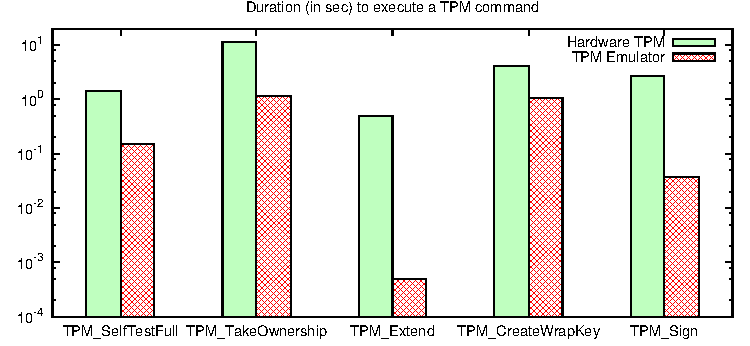
\includegraphics[width=.95\textwidth]{plots/performance_comparison}
			\end{center}
		\item[Result:] software emulation on average about \alert{\emph{ten times
			faster}},\\
			\textsf{TPM\_Extend} is even three orders of magnitude faster
	\end{description}
\end{frame}

\begin{frame}
	\frametitle{Performance Evaluation (2)}
	\begin{description}[]
		\item[Evaluation Environment:] Lenovo ThinkPad X61s (Intel Pentium
			Core 2 Duo 1.6\,GHz, 2 GB RAM), Linux 2.6.24, Atmel TPM v1.2
			\begin{center}
				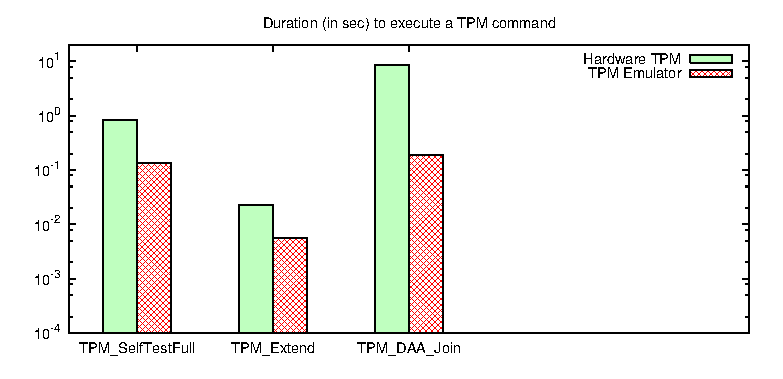
\includegraphics[width=.95\textwidth]{plots/performance_comparison2}
			\end{center}
		\item[Result:] computation-intensive commands
			\alert{\emph{hundred times faster}}
	\end{description}
\end{frame}

\section{Compliance Tests}

\begin{frame}
	\frametitle{Compliance Tests}
	\begin{description}[]
		\item[Compliance and Functionality Tests:]\hfill
			{\small\begin{itemize}
				\item IBM: TrouSerS (package \texttt{testsuite} and package \texttt{tpm-tools})
				\item TU Graz: jTSS (package \texttt{jTSS} and package \texttt{jTpmTools})
				\item IBM: DAA Test Suite (thanks to Roger Zimmermann)
				\item RU Bochum, Sirrix: TPM Test Suite (thanks to Marcel Selhorst)
			\end{itemize}}
	\end{description}
	\begin{center}
		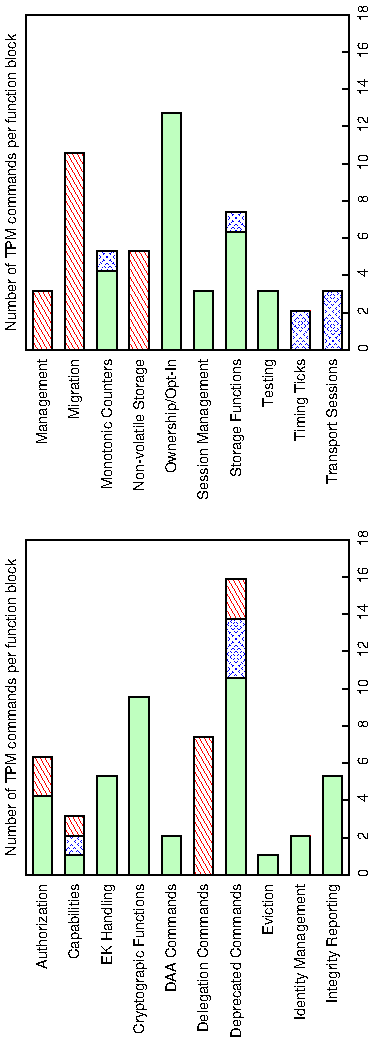
\includegraphics[angle=-90,scale=0.55]{plots/compliance}
		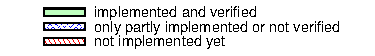
\includegraphics[origin=br,angle=90,scale=0.6]{plots/compliance_key}
	\end{center}
\end{frame}

\section{Conclusion}

\begin{frame}
	\frametitle{Conclusion}
	\begin{description}[]
		\item[Open Questions:]\hfill\\
			\begin{itemize}
				\item Performance evaluation: influence of LPC bus overhead
        \item Design and implement an interface for locality selection
			\end{itemize}\pause
		\item[Roadmap:]\hfill\\
			\begin{enumerate}
				\item Include changes from MTM Emulator (Nokia)
				\item Provide autoconf/automake build support
				\item Complete missing (mandatory) TPM commands
					\begin{itemize}
						\item Some capability areas and \textsf{TPM\_SetCapability}
						\item NV storage functions (Mario: next weeks)
						\item Migration and delegation functions
					\end{itemize}
				\item Add optional commands and algorithms (e.g. AES)
				\item Native support for other operating systems
			\end{enumerate}
	\end{description}
\end{frame}

\begin{frame}
	\frametitle{}
	\begin{center}
		\begin{Huge}
			\textbf{Thank you! Questions?}
		\end{Huge}
	\end{center}
\end{frame}

\section*{References}

\begin{frame}
	\frametitle{References}
	{\tiny\begin{thebibliography}{999999}
		%\beamertemplatetextbibitems
	\beamertemplatebookbibitems
		\bibitem{Mitchell2005}
			Chris Mitchell et~al.
			\newblock Trusted Computing.
			\newblock IET, 2005.
		\bibitem{Challener2008}
			David Challener, Kent Yoder, Ryan Catherman, David Safford, and
			Leendert Van Doorn.
			\newblock A Practical Guide to Trusted Computing.
			\newblock IBM Press, 2008.
		\bibitem{TPM}
			Trusted Computing Group.
			\newblock TPM Specification, Version 1.2, Revision 103.
			\newblock
			{\large\Keyboard}\hspace{2mm}\url{https://www.trustedcomputinggroup.org/specs/TPM/}.
	\beamertemplatearticlebibitems
		\bibitem{Sadeghi}
			Ahmad-Reza Sadeghi, Marcel Selhorst, Christian St\"{u}ble,
			Christian Wachsmann, and Marcel Winandy.
			\newblock TCG inside? A Note on TPM Specification Compliance.
			\newblock Proceedings of STC '06, pp. 47--56, 2006.
	%\beamertemplatetextbibitems
		\bibitem{TPMEmu}
			Mario Strasser et~al.
			\newblock Software-Based Trusted Platform Module Emulator.
			\newblock
			{\large\Keyboard}\hspace{2mm}\url{http://tpm-emulator.berlios.de/}.
		\bibitem{jTSS}
			TU Graz, IAIK.
			\newblock jTSS -- Java TCG Software Stack.
			\newblock
			{\large\Keyboard}\hspace{2mm}\url{http://trustedjava.sourceforge.net/}.
		\bibitem{trousers}
			Kent Yoder et~al.
			\newblock TrouSerS -- Open-source TCG Software Stack.
			\newblock
			{\large\Keyboard}\hspace{2mm}\url{http://trousers.sourceforge.net/}.
		\bibitem{ibmdaatest}
			Roger Zimmermann.
			\newblock IBM Direct Anonymous Attestation Tools -- TPM Test Suite.
			\newblock
			{\large\Keyboard}\hspace{2mm}\url{http://www.zurich.ibm.com/security/daa/}.
	\end{thebibliography}}
\end{frame}

\begin{frame}[fragile,allowframebreaks]
	\frametitle{Appendix: Supported TPM Commands}
	\definecolor{tpmgray}{gray}{0.85}
	\newcommand{\tpmred}{tpmgray!10!red!50!white}
	\newcommand{\tpmyellow}{tpmgray!10!yellow!50!white}
	\newcommand{\tpmgreen}{tpmgray!10!green!50!white}
	\newcommand{\tpmcolor}{tpmgray}
	\newcommand{\tpmcmd}[6]{
		\begin{tabular}{p{4.85cm}|p{0.46cm}|p{0.4cm}|p{0.25cm}|p{2.15cm}}
			\rowcolor{\tpmcolor}
				{\scriptsize\textsf{#1}} &
				{\scriptsize\textsf{#2}} &
				{\scriptsize\makebox[0.4cm][r]{#3}} &
				{\scriptsize\makebox[0.25cm][c]{#4}} &
				{\scriptsize #6}\\
		\end{tabular}
	}
	\newcommand{\tpmcmdr}[6]{
		\renewcommand{\tpmcolor}{\tpmred}
		\tpmcmd{#1}{#2}{#3}{#4}{#5}{#6}
		\renewcommand{\tpmcolor}{tpmgray}
	}
	\newcommand{\tpmcmdg}[6]{
		\renewcommand{\tpmcolor}{\tpmgreen}
		\tpmcmd{#1}{#2}{#3}{#4}{#5}{#6}
		\renewcommand{\tpmcolor}{tpmgray}
	}
	\newcommand{\tpmcmdy}[6]{
		\renewcommand{\tpmcolor}{\tpmyellow}
		\tpmcmd{#1}{#2}{#3}{#4}{#5}{#6}
		\renewcommand{\tpmcolor}{tpmgray}
	}
{\tiny
Admin Startup and State (pp. 5--10)\\
\tpmcmdg{TPM\_Init}{1.1}{151}{M}{tpm\_startup.c}{}\\
\tpmcmdg{TPM\_Startup}{1.1}{153}{M}{tpm\_startup.c}{}\\
\tpmcmdg{TPM\_SaveState}{1.1}{152}{M}{tpm\_startup.c}{}\\
Admin Testing (pp. 11--14)\\
\tpmcmdg{TPM\_SelfTestFull}{1.1}{80}{M}{tpm\_testing.c}{passed \cite{trousers,jTSS}}\\
\tpmcmdg{TPM\_ContinueSelfTest}{1.1}{83}{M}{tpm\_testing.c}{}\\
\tpmcmdg{TPM\_GetTestResult}{1.1}{84}{M}{tpm\_testing.c}{passed \cite{trousers,jTSS}}\\
Admin Opt-in (pp. 15--22)\\
\tpmcmdg{TPM\_SetOwnerInstall}{1.1}{113}{M}{tpm\_owner.c}{}\\
\tpmcmdg{TPM\_OwnerSetDisable}{1.1}{110}{M}{tpm\_owner.c}{}\\
\tpmcmdg{TPM\_PhysicalEnable}{1.1}{111}{M}{tpm\_owner.c}{}\\
\tpmcmdg{TPM\_PhysicalDisable}{1.1}{112}{M}{tpm\_owner.c}{}\\
\tpmcmdg{TPM\_PhysicalSetDeactivated}{1.1}{114}{M}{tpm\_owner.c}{}\\
\tpmcmdg{TPM\_SetTempDeactivated}{1.1}{115}{M}{tpm\_owner.c}{}\\
\tpmcmdg{TPM\_SetOperatorAuth}{1.2}{116}{M}{tpm\_owner.c}{}\\
Admin Ownership (pp. 23--36)\\
\tpmcmdg{TPM\_TakeOwnership}{1.1}{13}{M}{tpm\_owner.c}{passed \cite{trousers,jTSS}}\\
\tpmcmdg{TPM\_OwnerClear}{1.1}{91}{M}{tpm\_owner.c}{}\\
\tpmcmdg{TPM\_ForceClear}{1.1}{93}{M}{tpm\_owner.c}{}\\
\tpmcmdg{TPM\_DisableOwnerClear}{1.1}{92}{M}{tpm\_owner.c}{}\\
\tpmcmdg{TPM\_DisableForceClear}{1.1}{94}{M}{tpm\_owner.c}{}\\
\tpmcmdg{TSC\_PhysicalPresence}{1.1}{}{M}{tpm\_owner.c}{}\\
\tpmcmdg{TSC\_ResetEstablishmentBit}{1.2}{}{M}{tpm\_owner.c}{}\\
Capability Commands (pp. 37--42)\\
\tpmcmdy{TPM\_GetCapability}{1.1}{101}{M}{tpm\_capability.c}{TODO: 45\,\%}\\
\tpmcmdr{TPM\_SetCapability}{1.2}{63}{M}{tpm\_capability.c}{}\\
\tpmcmdg{TPM\_GetCapabilityOwner}{1.1}{102}{M}{tpm\_capability.c}{}\\
Auditing (pp. 43--51)\\
\tpmcmdg{TPM\_GetAuditDigest}{1.2}{133}{O}{tpm\_audit.c}{failed \cite{trousers}}\\
\tpmcmdg{TPM\_GetAuditDigestSigned}{1.2}{134}{O}{tpm\_audit.c}{}\\
\tpmcmdg{TPM\_SetOrdinalAuditStatus}{1.1}{141}{O}{tpm\_audit.c}{}\\
Administrative Functions -- Management (pp. 52--57)\\
\tpmcmdr{TPM\_FieldUpgrade}{1.1}{170}{O}{tpm\_management.c}{}\\
\tpmcmdr{TPM\_SetRedirection}{1.1}{154}{O}{tpm\_management.c}{}\\
\tpmcmdr{TPM\_ResetLockValue}{1.2}{64}{M}{tpm\_management.c}{}\\
Storage Functions (pp. 58--81)\\
\tpmcmdg{TPM\_Seal}{1.1}{23}{M}{tpm\_storage.c}{passed \cite{trousers,jTSS,Sadeghi}}\\
\tpmcmdg{TPM\_Unseal}{1.1}{24}{M}{tpm\_storage.c}{passed \cite{jTSS}}\\
\tpmcmdg{TPM\_UnBind}{1.1}{30}{M}{tpm\_storage.c}{passed \cite{trousers,jTSS,Sadeghi}}\\
\tpmcmdg{TPM\_CreateWrapKey}{1.1}{31}{M}{tpm\_storage.c}{passed \cite{trousers,jTSS,Sadeghi}}\\
\tpmcmdy{TPM\_LoadKey2}{1.2}{65}{M}{tpm\_storage.c}{emulated by 32}\\
\tpmcmdg{TPM\_GetPubKey}{1.1}{33}{M}{tpm\_storage.c}{passed \cite{trousers}}\\
\tpmcmdr{TPM\_Sealx}{1.2}{61}{O}{tpm\_storage.c}{}\\
Migration (pp. 82--108)\\
\tpmcmdr{TPM\_CreateMigrationBlob}{1.1}{40}{M}{tpm\_migration.c}{}\\
\tpmcmdr{TPM\_ConvertMigrationBlob}{1.1}{42}{M}{tpm\_migration.c}{}\\
\tpmcmdr{TPM\_AuthorizeMigrationKey}{1.1}{43}{M}{tpm\_migration.c}{}\\
\tpmcmdr{TPM\_MigrateKey}{1.2}{37}{M}{tpm\_migration.c}{}\\
\tpmcmdr{TPM\_CMK\_SetRestrictions}{1.2}{28}{M}{tpm\_migration.c}{}\\
\tpmcmdr{TPM\_CMK\_ApproveMA}{1.2}{29}{M}{tpm\_migration.c}{}\\
\tpmcmdr{TPM\_CMK\_CreateKey}{1.2}{19}{M}{tpm\_migration.c}{}\\
\tpmcmdr{TPM\_CMK\_CreateTicket}{1.2}{18}{M}{tpm\_migration.c}{}\\
\tpmcmdr{TPM\_CMK\_CreateBlob}{1.2}{27}{M}{tpm\_migration.c}{}\\
\tpmcmdr{TPM\_CMK\_ConvertMigration}{1.2}{36}{M}{tpm\_migration.c}{}\\
Maintenance Functions (optional, pp. 109--118)\\
\tpmcmdr{TPM\_CreateMaintenanceArchive}{1.1}{44}{O}{tpm\_maintenance.c}{}\\
\tpmcmdr{TPM\_LoadMaintenanceArchive}{1.1}{45}{O}{tpm\_maintenance.c}{}\\
\tpmcmdr{TPM\_KillMaintenanceFeature}{1.1}{46}{O}{tpm\_maintenance.c}{}\\
\tpmcmdr{TPM\_LoadManuMaintPub}{1.1}{47}{O}{tpm\_maintenance.c}{}\\
\tpmcmdr{TPM\_ReadManuMaintPub}{1.1}{48}{O}{tpm\_maintenance.c}{}\\
Cryptographic Functions (pp. 119--136)\\
\tpmcmdg{TPM\_SHA1Start}{1.1}{160}{M}{tpm\_crypto.c}{passed \cite{trousers,jTSS}}\\
\tpmcmdg{TPM\_SHA1Update}{1.1}{161}{M}{tpm\_crypto.c}{passed \cite{trousers,jTSS}}\\
\tpmcmdg{TPM\_SHA1Complete}{1.1}{162}{M}{tpm\_crypto.c}{passed \cite{trousers,jTSS}}\\
\tpmcmdg{TPM\_SHA1CompleteExtend}{1.1}{163}{M}{tpm\_crypto.c}{passed \cite{trousers}}\\
\tpmcmdg{TPM\_Sign}{1.1}{60}{M}{tpm\_crypto.c}{passed \cite{trousers,jTSS,Sadeghi}}\\
\tpmcmdg{TPM\_GetRandom}{1.1}{70}{M}{tpm\_crypto.c}{passed \cite{trousers,jTSS,Sadeghi}}\\
\tpmcmdg{TPM\_StirRandom}{1.1}{71}{M}{tpm\_crypto.c}{passed \cite{trousers,jTSS}}\\
\tpmcmdg{TPM\_CertifyKey}{1.1}{50}{M}{tpm\_crypto.c}{passed \cite{trousers,jTSS}}\\
\tpmcmdg{TPM\_CertifyKey2}{1.2}{51}{M}{tpm\_crypto.c}{}\\
Endorsement Key Handling (pp. 137--145)\\
\tpmcmdy{TPM\_CreateEndorsementKeyPair}{1.1}{120}{M}{tpm\_credentials.c}{disabled}\\
\tpmcmdg{TPM\_CreateRevocableEK}{1.2}{127}{O}{tpm\_credentials.c}{}\\
\tpmcmdg{TPM\_RevokeTrust}{1.2}{128}{O}{tpm\_credentials.c}{}\\
\tpmcmdg{TPM\_ReadPubek}{1.1}{124}{M}{tpm\_credentials.c}{passed \cite{trousers,jTSS}}\\
\tpmcmdg{TPM\_OwnerReadInternalPub}{1.2}{129}{M}{tpm\_credentials.c}{}\\
Identity Creation and Activation (pp. 146--152)\\
\tpmcmdg{TPM\_MakeIdentity}{1.1}{121}{M}{tpm\_identity.c}{passed \cite{trousers,jTSS}}\\
\tpmcmdg{TPM\_ActivateIdentity}{1.1}{122}{M}{tpm\_identity.c}{passed \cite{trousers,jTSS}}\\
Integrity Collection and Reporting (pp. 153--163)\\
\tpmcmdg{TPM\_Extend}{1.1}{20}{M}{tpm\_integrity.c}{passed \cite{trousers,jTSS}}\\
\tpmcmdg{TPM\_PCRRead}{1.1}{21}{M}{tpm\_integrity.c}{passed \cite{trousers,jTSS,Sadeghi}}\\
\tpmcmdg{TPM\_Quote}{1.1}{22}{M}{tpm\_integrity.c}{passed \cite{trousers,jTSS}}\\
\tpmcmdg{TPM\_PCR\_Reset}{1.2}{200}{M}{tpm\_integrity.c}{not supported \cite{jTSS}}\\
\tpmcmdg{TPM\_Quote2}{1.2}{62}{M}{tpm\_integrity.c}{passed \cite{trousers}}\\
Changing AuthData (pp. 164--168)\\
\tpmcmdg{TPM\_ChangeAuth}{1.1}{12}{M}{tpm\_authorization.c}{passed \cite{trousers}}\\
\tpmcmdg{TPM\_ChangeAuthOwner}{1.1}{16}{M}{tpm\_authorization.c}{}\\
Authorization Sessions (pp. 169--181)\\
\tpmcmdg{TPM\_OIAP}{1.1}{10}{M}{tpm\_authorization.c}{not random \cite{Sadeghi}}\\
\tpmcmdg{TPM\_OSAP}{1.1}{11}{M}{tpm\_authorization.c}{not random \cite{Sadeghi}}\\
\tpmcmdr{TPM\_DSAP}{1.2}{17}{M}{tpm\_authorization.c}{}\\
\tpmcmdy{TPM\_SetOwnerPointer}{1.2}{117}{M}{tpm\_authorization.c}{disabled}\\
Delegation Commands (pp. 182--201)\\
\tpmcmdr{TPM\_Delegate\_Manage}{1.2}{210}{M}{tpm\_delegation.c}{}\\
\tpmcmdr{TPM\_Delegate\_CreateKeyDelegation}{1.2}{212}{M}{tpm\_delegation.c}{}\\
\tpmcmdr{TPM\_Delegate\_CreateOwnerDelegation}{1.2}{213}{M}{tpm\_delegation.c}{}\\
\tpmcmdr{TPM\_Delegate\_LoadOwnerDelegation}{1.2}{216}{M}{tpm\_delegation.c}{}\\
\tpmcmdr{TPM\_Delegate\_ReadTable}{1.2}{219}{M}{tpm\_delegation.c}{}\\
\tpmcmdr{TPM\_Delegate\_UpdateVerification}{1.2}{209}{M}{tpm\_delegation.c}{}\\
\tpmcmdr{TPM\_Delegate\_VerifyDelegation}{1.2}{214}{M}{tpm\_delegation.c}{}\\
Non-volatile Storage (pp. 202--215)\\
\tpmcmdr{TPM\_NV\_DefineSpace}{1.2}{204}{M}{tpm\_nv\_storage.c}{}\\
\tpmcmdr{TPM\_NV\_WriteValue}{1.2}{205}{M}{tpm\_nv\_storage.c}{}\\
\tpmcmdr{TPM\_NV\_WriteValueAuth}{1.2}{206}{M}{tpm\_nv\_storage.c}{}\\
\tpmcmdr{TPM\_NV\_ReadValue}{1.2}{207}{M}{tpm\_nv\_storage.c}{}\\
\tpmcmdr{TPM\_NV\_ReadValueAuth}{1.2}{208}{M}{tpm\_nv\_storage.c}{}\\[3mm]
Session Management (pp. 216--223)\\
\tpmcmdg{TPM\_KeyControlOwner}{1.2}{35}{M}{tpm\_context.c}{failed \cite{trousers}}\\
\tpmcmdg{TPM\_SaveContext}{1.2}{184}{M}{tpm\_context.c}{}\\
\tpmcmdg{TPM\_LoadContext}{1.2}{185}{M}{tpm\_context.c}{}\\
Eviction (pp. 224--226)\\
\tpmcmdy{TPM\_FlushSpecific}{1.2}{186}{M}{tpm\_eviction.c}{TODO: 75\,\%}\\
Timing Ticks (pp. 227--230)\\
\tpmcmdg{TPM\_GetTicks}{1.2}{241}{M}{tpm\_ticks.c}{failed \cite{trousers,jTSS}}\\
\tpmcmdg{TPM\_TickStampBlob}{1.2}{242}{M}{tpm\_ticks.c}{failed \cite{trousers,jTSS}}\\
Transport Sessions (pp. 231--244)\\
\tpmcmdg{TPM\_EstablishTransport}{1.2}{230}{M}{tpm\_transport.c}{failed \cite{trousers}}\\
\tpmcmdg{TPM\_ExecuteTransport}{1.2}{231}{M}{tpm\_transport.c}{failed \cite{trousers}}\\
\tpmcmdg{TPM\_ReleaseTransportSigned}{1.2}{232}{M}{tpm\_transport.c}{failed \cite{trousers}}\\
Monotonic Counter (pp. 245--254)\\
\tpmcmdg{TPM\_CreateCounter}{1.2}{220}{M}{tpm\_counter.c}{passed \cite{Sadeghi}}\\
\tpmcmdg{TPM\_IncrementCounter}{1.2}{221}{M}{tpm\_counter.c}{passed \cite{Sadeghi}}\\
\tpmcmdg{TPM\_ReadCounter}{1.2}{222}{M}{tpm\_counter.c}{passed \cite{Sadeghi}, failed \cite{trousers}}\\
\tpmcmdg{TPM\_ReleaseCounter}{1.2}{223}{M}{tpm\_counter.c}{passed \cite{Sadeghi}}\\
\tpmcmdg{TPM\_ReleaseCounterOwner}{1.2}{224}{M}{tpm\_counter.c}{}\\
DAA Commands (pp. 255--282)\\
\tpmcmdg{TPM\_Join}{1.2}{41}{M}{tpm\_daa.c}{passed \cite{ibmdaatest}}\\
\tpmcmdg{TPM\_Sign}{1.2}{49}{M}{tpm\_daa.c}{passed \cite{ibmdaatest}}\\
Deprecated Commands (pp. 283--309)\\
\tpmcmdg{TPM\_EvictKey}{1.1}{34}{D}{tpm\_deprecated.c}{}\\
\tpmcmdg{TPM\_Terminate\_Handle}{1.1}{150}{D}{tpm\_deprecated.c}{}\\
\tpmcmdg{TPM\_SaveKeyContext}{1.1}{180}{D}{tpm\_deprecated.c}{}\\
\tpmcmdg{TPM\_LoadKeyContext}{1.1}{181}{D}{tpm\_deprecated.c}{}\\
\tpmcmdg{TPM\_SaveAuthContext}{1.1}{182}{D}{tpm\_deprecated.c}{}\\
\tpmcmdg{TPM\_LoadAuthContext}{1.1}{183}{D}{tpm\_deprecated.c}{}\\
\tpmcmdg{TPM\_DirWriteAuth}{1.1}{25}{D}{tpm\_deprecated.c}{passed \cite{trousers,jTSS}}\\
\tpmcmdg{TPM\_DirRead}{1.1}{26}{D}{tpm\_deprecated.c}{passed \cite{trousers,jTSS}}\\
\tpmcmdg{TPM\_ChangeAuthAsymStart}{1.1}{14}{D}{tpm\_deprecated.c}{}\\
\tpmcmdg{TPM\_ChangeAuthAsymFinish}{1.1}{15}{D}{tpm\_deprecated.c}{}\\
\tpmcmdg{TPM\_Reset}{1.1}{90}{D}{tpm\_deprecated.c}{}\\
\tpmcmdg{TPM\_OwnerReadPubek}{1.1}{125}{D}{tpm\_deprecated.c}{}\\
\tpmcmdg{TPM\_DisablePubekRead}{1.1}{126}{?}{tpm\_credentials.c}{spec error?}\\
\tpmcmdg{TPM\_LoadKey}{1.1b}{32}{D}{tpm\_storage.c}{passed \cite{trousers,jTSS}}\\
Deleted Commands (pp. 310--314)\\
\tpmcmdr{TPM\_GetCapabilitySigned}{1.1}{100}{X}{}{}\\
\tpmcmdr{TPM\_GetOrdinalAuditStatus}{1.1}{140}{X}{}{}\\
\tpmcmdg{TPM\_CertifySelfTest}{1.1}{82}{X}{tpm\_deprecated.c}{bad ordinal~\cite{trousers}}\\
\tpmcmdr{TPM\_GetAuditEventSigned}{1.1}{130}{X}{}{}\\
\tpmcmdr{TPM\_GetAuditEventSigned}{1.1}{131}{X}{}{}\par
}
\vfill
~
\end{frame}

\end{document}
